\documentclass[sigconf,review]{acmart}\settopmatter{printfolios=true}
% \documentclass[review]{acmart}\settopmatter{printfolios=true}

\usepackage{amssymb}
\usepackage{amsthm}
\usepackage{graphicx}
\usepackage{amsmath}
\usepackage{mathptmx}
\usepackage{mathtools}
\usepackage{stmaryrd}
\usepackage{hyperref}
\usepackage{alltt}
\usepackage{url}
\usepackage{float}
\usepackage{style/utils}
\usepackage{style/code}
\usepackage{style/proof}
\usepackage{style/keywords}
\usepackage{style/layout}
\usepackage{style/judgements}

% for combinator pictures
\usepackage{tikz}
\usepackage{pgfplots}
\usetikzlibrary{shapes,arrows}
\usepackage[outputdir={out/}]{dot2texi}

\setcopyright{none}
\bibliographystyle{ACM-Reference-Format}
% \citestyle{acmauthoryear}

% -----------------------------------------------------------------------------
\begin{document}

\title{Machine Fusion}
\subtitle{Merging merges, more or less}

\author{Amos Robinson}
\affiliation{Ambiata and UNSW (Australia)}
\email{amosr@cse.unsw.edu.au}

\author{Ben Lippmeier}
\affiliation{Digital Asset and UNSW (Australia)}
\email{benl@ouroborus.net}

\makeatactive
\begin{abstract}
Compilers for stream programs often rely on a fusion transformation to convert the implied dataflow network into low-level iteration based code. Different fusion transformations handle different sorts of networks, with the distinguishing criteria being whether the network may contain splits and joins, and whether the set of fusible operators can be extended. We present the first fusion system that simultaneously satisfies all three of these criteria: networks can contain splits and joins, and new operators can be added to the system without needing to modify the overall fusion transformation.
% Our system has been formalized in Coq, and we have proved soundness of the core transformation.
\end{abstract}


\maketitle

%!TEX root = ../Main.tex
\section{Introduction}
\label{s:Introduction}

Suppose we have two input streams of numeric identifiers, and wish to perform some analysis on these identifiers. The identifiers from both streams arrive sorted, but may include duplicates. We wish to produce an output stream of unique identifiers from the first input stream, as well as produce the unique union of identifiers from both streams. Can we perform both of these tasks at once, without needing to read through the stream data multiple times, and without needing unbounded buffering? Here is how we might write the source code, where @S@ is for @S@-tream.
\begin{code}
  uniquesUnion : S Nat -> S Nat -> (S Nat, S Nat)
  uniquesUnion sIn1 sIn2
   = let  sUnique = group sIn1
          sMerged = merge sIn1 sIn2
          sUnion  = group sMerged
     in   (sUnique, sUnion)
\end{code}

In this implementation the @group@ operator filters out consecutive duplicates, while @merge@ combines two sorted streams so that the output remains sorted. This example has a few interesting properties. Firstly, the data-access pattern of @merge@ is \emph{value-dependent}, meaning that the order in which this operator pulls values from @sIn1@ and @sIn2@ depends on the values themselves. If all the values from @sIn1@ are smaller than the values in @sIn2@, then @merge@ will pull all values from @sIn1@ before pulling the rest from @sIn2@, and vice versa. Secondly, although @sIn1@ occurs twice in the program, at runtime we only want to handle the elements of each stream once. To achieve this, the compiled program must coordinate between the two uses of @sIn1@, so that values are only read when both the @group@ and @merge@ operators are ready to receive a new value. Finally, as the stream length is assumed to be unbounded, we cannot buffer an arbitrary number of elements read from either stream, or risk running out of local storage space.

For an implementation which does \emph{not} use stream fusion, we might implement each of the operators as a separate concurrent process, and send each identifier value using an intra-process communication mechanism. Developing such an implementation could be easy or hard, depending on what language features are available for concurrency. However, worrying about the \emph{performance tuning} of such a system, such as whether we need back-pressure, or how to chunk the stream data to reduce the amount of communication overhead, is invariably a headache. 

We might instead define some sort of uniform interface for data sources, with a single `pull' function that provides the next value in each stream. Each operator could be given this interface, so that the next value from each result stream is computed on demand. This is approach is commonly taken with implementations of physical operators in data base systems. However, this `pull only' model does not support operators with multiple outputs, such as our derived @uniquesUnion@ operator, at least not without unbounded buffering. Suppose a consumer pulls many elements from the result @sUnique@ stream. The implementation needs to pull the corresponding source elements from @sIn1@ \emph{as well} as buffering an arbitrary number of matching elements from @sIn2@. It needs to buffer an aribrary number of elements from @sIn2@ because there is no guarantee of when a consumer will also pull from the @sUnion@ result stream. Once that happens the elements from @sIn2@ no longer need to be retained, but not before.

Instead, for a single threaded program, we want to perform \emph{stream fusion}, which takes the dataflow network and produces a simple sequential loop that gets the job done without requiring extra process-control abstractions and without requiring unbounded buffering. Sadly, existing stream fusion transformations cannot handle our example. As observed by \citet{kay2009you}, both pull-based and push-based fusion have fundamental limitations. Pull-based systems such as short cut stream fusion~\cite{coutts2007stream} cannot handle cases where a particular stream or intermediate result is used by multiple consumers. We refer to this situation as a \mbox{\emph{split} --- in the} dataflow network the flow from input stream @sIn1@ is split into both the @group@ and @merge@ consumers. 

% Leave this to related work. We've already mentioned a canonical pull-based system.
% Recent work on stream fusion by \citet{kiselyov2016stream} uses staged computation to ensure all combinators are inlined, but for splits this causes excessive inlining which duplicates work, due to values of the source arrays being read multiple times.

Push-based systems such as foldr/build fusion~\cite{gill1993short} also cannot fuse our example because they do not support operators with multiple inputs. We refer to such a situation as a \emph{join} --- in our example the @merge@ operator expresses a join in the data-flow graph. Some systems support both pull and push: data flow inspired array fusion~\cite{lippmeier2013data} allows both splits and joins but only for a limited, predefined set of operators. More recent work on polarized data flow fusion~\cite{lippmeier2016polarized} \emph{is} able to fuse our example, but requires the program to be rewritten to use explicitly polarized stream types. 

% The mechanism that combines the implementations of both operators, to yield efficient imperative code also depends on the general purpose compiler optimisations implemented by GHC, and it can be difficult to tell if these have ``worked'' without inspecting the intermediate representations of the compiler.

Synchronous dataflow languages such as Lucy-n~\cite{mandel2010lucy} reject value-dependent operators such as @merge@, while general dataflow languages fall back on less performant dynamic scheduling for these cases \cite{bouakaz2013real}. The polyhedral array fusion model~\cite{feautrier2011polyhedron} is used for loop transformations in imperative programs, but operates at a much lower level. The polyhedral model is based around affine loops, which makes it difficult to support filter-like operators such as @group@ and @merge@.

In our new system we still view the program as a concurrent process network. Each operator is a separate process, and the stream data flows through communication channels between the processes. Each operator is expressed as a restricted, sequential imperative program with commands that include both @pull@ for reading from an input stream and @push@ for writing to an output stream. The fusion transform takes the concurrent process network and \emph{sequentializes} it into a single process by choosing a particular evaluation order that requires no unbounded intermediate buffers. When the fusion transformation succeeds we know it has worked. There is no need to inspect intermediate representations of the compiler to debug poor performance, which is a common problem in systems based on general purpose program transformations \cite{lippmeier2012:guiding}.

In summary, we make the following contributions:
\begin{itemize}
\item a process calculus for encoding infinite streaming programs (\S\ref{s:Processes});
\item an algorithm for fusing these processes, the first to support arbitrary splits and joins (\S\ref{s:Fusion});
\item numerical results that demonstrate that the algorithm is well behaved when the number of fused processes is large. The size of the fused result program is not excessive. \TODO{Ref}
\item a formalization and proof of soundness for the core fusion algorithm in Coq (\S\ref{s:Proofs});
\end{itemize}

Our fusion transformation for infinite stream programs could also serve as the basis for an \emph{array} fusion system, using a natural extension to finite streams. We discuss this extension in \S\ref{s:Finite}.

% TODO: We can't make the appendix a contribution because the reviewers are not required to read appendices.
% \item and show our processes are general enough for many combinators, including segmented operations (\S\ref{s:Combinators}).

% \ben{Add a few more sentences on related work. Explain how this work extends the old flow fusion paper. It is not short-cut fusion like Oleg's recent work. We are not in the same space as Fortran style array fusion transformations like polyhedral}

% BL: describe this later.
% Furthermore, the data-flow fusion system of~\cite{lippmeier2013data} only deals with a fixed set of baked-in combinators. 

% BL: Shift the detailed description into a later section.
% The example above has three combinators, so the process network has three processes.
% The two @writeFile@s outputs are treated as sinks that values can be pushed to at any time, and are not converted to processes.
% During code generation, any output values from the @uniques@ and @union@ streams are sent to the corresponding @writeFile@ sink, but we do not address code generation in this paper.

% The process for @uniques@ is defined by the @group@ combinator, and can be thought of as an imperative loop: first it reads from its input stream @file1@ and stores that in a local variable.
% It also keeps track of the last pulled value, and compares that against the newly read value.
% If they are different, it pushes the new value to its output stream @uniques@.
% In either case, it updates the last pulled value and loops back to the start to pull from @file1@ again.

% The process for @merged@ is defined by the @merge@ combinator, which starts by reading from both @file1@ and @file2@ and storing these in local variables.
% It then compares its two values to see which is the smaller.
% If the value from @file1@ is smaller, it pushes that value and pulls a new value from @file1@, otherwise it pushes the value from @file2@ and pulls from @file2@.
% This is performed in a loop.

% We fuse these two processes by interleaving the two such that the shared input @file1@ is only pulled from when both processes agree.
% The new process pulls from @file1@, which is copied to the variables for both processes.
% The @uniques@ process now has all it needs to execute, so it checks the value against the last pulled value, pushes if necessary, and goes back to try to pull from @file1@ again.
% At this stage the @merged@ process still has a value from @file1@ that it has pulled but not used, so @uniques@ cannot pull from @file1@ again.
% We now let @merged@ run, pulling from @file2@ and checking which is smaller.
% If the value from @file1@ is smaller, the value is emitted and @merged@ wishes to pull a new value from @file1@.
% Both processes now agree on pulling from @file1@ again, so the new value is pulled and @uniques@ can run again.
% Otherwise if the value from @file1@ is not smaller, the value from @file2@ is emitted and @merged@ pulls from @file2@ with no coordination required.

% If we wish to ensure that each value is only read from the file once, we must coordinate between the two use sites: when @uniques@ requires a new value it must ensure that @union@ is ready to receive a new value, and vice versa. Note that we cannot just execute @uniques@ while storing the read values in a buffer, as this may require more memory than is available.
% In order to fuse this example, we require both pull \emph{and} push streams.
% The input streams must be pull streams since the order values are required is determined by the @merge@ combinator.
% For the same reason, the outputs sent to each @writeFile@ must be push streams.

% Fusion for array programs is important for removing intermediate arrays, reducing memory traffic and reducing allocations.
% However, when dealing with data too large to fit in memory such as tables on disk, removing intermediate arrays becomes essential rather than just desirable.
% Attempting to create an intermediate array of such amounts of data would lead to thrashing and swapping to disk, or perhaps even running out of swap.
% For these situations, some sort of assurance of total fusion is required: either the program can be fused with no intermediate arrays or unbounded buffers, or it will not compile at all.


% Fusion eliminates intermediate array buffers and converts pipelines of array combinators into low-level iteration based loop code. Different fusion systems can handle 

% When comparing fusion systems, three important criteria to consider are: whether the system supports splits, where a stream is used multiple times; whether it supports joins, where a combinator has multiple inputs; and whether arbitrary combinators such as @merge@ and segmented appends can be encoded. Existing fusion systems support one or two of these, but not three. We present a fusion system based on process calculus that supports all three: splits, joins and arbitrary combinators.

% Our system has been formalised in Coq where we have proved soundness of the fusion algorithm. It is expressive enough to encode a wide range of combinators including operations on segmented arrays.

% \amos{``Arbitrary combinators'' is not quite true. How can we distinguish combinators we support from 2013 data flow fusion paper? Perhaps by mentioning value-dependent input / access patterns.}

% Leave this to the description of the algorithm, not the abstract.
% We encode each combinator as a separate process with any number of input and output channels. Each process is sequential but multiple processes can be executed concurrently. We give a concurrent execution semantics for multiple processes, but these are used only as a specification for how the fused program must behave. The fused program itself is sequential and can easily be converted to simple imperative code.

% Our fusion algorithm takes two concurrently executable processes and creates a sequential interleaving of the two such that they execute with no unbounded buffers.
% If fusion would require unbounded buffers (or the fusion algorithm wrongly infers that it would) then fusion fails.
% If fusion fails, the user can be presented with an error message telling them which combinators could not be fused.
% For scenarios where fusion is required, this is a great advantage over fragile shortcut fusion systems.

% BL: leave the apologies to the conclusion.
% The version presented here deals with infinite streams, and we informally describe the extensions required to support finite streams.

% BL: leave this to the main intro.
% optimising high-level array and streaming computations, as it reduces memory traffic and intermediate arrays. The benefits of removing intermediate arrays are even more important as data sizes approach the size of memory.

%!TEX root = ../Main.tex

% -----------------------------------------------------------------------------
\section{Processes, Machines, Combinators and Operators}
\label{s:Processes}

A \emph{process} in our system is a simple imperative program with a local heap. A process pulls source values from an arbitrary number of input streams and pushes result values to at least one output stream. The process language is an intermediate representation we use when fusing the overall dataflow network. When describing the fusion transform we describe the control flow of the process as a state machine, hence Machine Fusion. 

A \emph{combinator} is a template for a particular process which parameterizes it over the particular input and output streams, as well as values of configuration parameters such as the worker function used in a @map@ process. Each process implements a logical \emph{operator} --- so we use ``operator'' when describing the values being computed, but ``process'' and ``machine'' when referring to the implementation. 


% -----------------------------------------------------------------------------
\subsection{Grouping}

The definition of the @group@ combinator which detects groups of successive identical elements in the input stream is given in Fig.~\ref{fig:Process:Group}. The process emits the first value pulled from the stream and every value that is different from the last one that was pulled. For example, when executed on the input stream @[1,2,2,3]@, the process will produce the output @[1,2,3]@. We include the concrete representation and a diagram of the process viewed as a state machine.

The @group@ combinator has two parameters, @sIn1@ and @sOut1@, which bind the input and output streams respectively. The \emph{nu-binders} \mbox{$\nu$ @(f: Bool) (l: Nat)@...} indicate that each time the @group@ combinator is instantiated, fresh names must be given to @f@, @l@ and so on, that do not conflict with other instantiations. Overall, the @f@ variable tracks whether we are dealing with the first value from the stream, @l@ holds the last value pulled from the stream (or 0 if none have been read yet), and @v@ holds the current value pulled from the stream. 

The body of the combinator is a record that defines the process. The @ins@ field of the record defines the set of input streams and the @outs@ field the set of output streams. The @heap@ field gives the initial values of each of the local variables. The @instrs@ field contains a set of labeled instructions that define the program, while the @label@ field gives the label of the initial instruction. Note that in this form the output stream is defined via a parameter, rather than being the result of the combinator, as in the source representation of @uniquesUnion@ from \S\ref{s:Introduction}. 

The initial instruction @(pull sIn1 v A1 [])@ pulls the next element from the stream @sIn1@, writes it into the heap variable @v@ (value), then proceeds to the instruction at label @A1@. The empty list @[]@ after the target label @A1@ can be used to update heap variables, but as we do not need to update anything yet we leave it empty. 

Next, the instruction @(case (f || (l /= v)) A2 [] A3 [])@ checks whether predicate @(f || (l /= v))@ is true; if so it proceeds to the instruction at label @A2@, otherwise it proceeds to @A3@. We use the variable @l@ (last) to track the last value read from the stream, and the boolean @f@ (first) to track whether this is the first element.

When the predicate is true, the instruction @(push sOut1 v A3 [ l = v, f = F ])@ pushes the value @v@ to the output stream @sOut1@ and proceeds to the instruction at label @A3@, once the variable @l@ is set to @v@ and @f@ to @F@ (False).

Finally, the instruction @(drop sIn1 A0 [])@ signals that the current element that was pulled from stream @sIn1@ is no longer required, and goes back to the first the instruction at @A0@. This @drop@ instruction is used to coordinate concurrent processes when performing fusion. The next element of a stream may only be pulled after all consumers of that stream have pulled and then and dropped the current element.


\begin{figure*}

\begin{center}
\begin{alltt}
           group 
             = \(\lambda\) (sIn1: Stream Nat) (sOut1: Stream Nat). 
               \(\nu\) (f: Bool) (l: Nat) (v: Nat) (A0..A3: Label).
\end{alltt}
\begin{code}
               process
                { ins:    { sIn1  }
                , outs:   { sOut1 }
                , heap:   { f = T, l = 0, v = 0 }
                , label:  A0
                , instrs: { A0 = pull sIn1 v          A1 []
                          , A1 = case (f || (l /= v)) A2 []  A3 []
                          , A2 = push sOut1 v         A3 [ l = v, f = F ]
                          , A3 = drop sIn1            A0 [] } }
\end{code}
\end{center}
\vspace{1em}
\includegraphics[scale=1.1]{figures/state-group.pdf}
\caption{The group combinator}
\label{fig:Process:Group}
\end{figure*}


% -----------------------------------------------------------------------------
\subsection{Merging}
\begin{figure*}
\begin{alltt}
               merge
                 = \(\lambda\) (sIn1: Stream Nat) (sIn2: Stream Nat) (sOut2: Stream Nat). 
                   \(\nu\) (x1: Nat) (x2: Nat) (B0..E2: Label).
\end{alltt}
\begin{code}
                   process
                    { ins:    { sM1, sM2 }
                    , outs:   { sM3 }
                    , heap:   { x1 = 0, x2 = 0 }
                    , label:  B0
                    , instrs: { B0 = pull sIn1  x1   B1 []
                              , B1 = pull sIn2  x2   C0 []
                              , C0 = case (x1 < x2)  D0 []  E0 []
                              , D0 = push sOut2 x1   D1 []
                              , D1 = drop sIn1       D2 []
                              , D2 = pull sIn1  x1   C0 []
                              , E0 = push sOut2 x2   E1 []
                              , E1 = drop sIn2       E2 []
                              , E2 = pull sIn2 x2    C0 [] } }
\end{code}

\medskip
\includegraphics[scale=1.1]{figures/state-merge.pdf}
\caption{The merge combinator}
\label{fig:Process:Merge}
\end{figure*}

The definition of the @merge@ combinator, which merges two input streams, is given in Fig.~\ref{fig:Process:Merge}. The combinator binds the two input streams to @sIn1@ and @sIn2@, while the output stream is @sOut2@. The two heap variables @x1@ and @x2@ are used to store the last values read from each input stream. The process starts by pulling from each of the input streams. It then compares the two pulled values, and pushes the smaller of the values to the output stream. The process then drops the stream which yielded the the smaller value, then pulls from the same stream so that it can perform the comparison again.

As the @merge@ process merges infinite streams, if we execute it with a finite input prefix, it will arrive at an intermediate state that may not yet have pushed all available output. For example, if we execute the process with the input streams @[1,4]@ and @[2,3,100]@ then the values @[1,2,3,4]@ will be pushed to the output. After pushing the last value @4@, the process will block at instruction @E2@, waiting for the next value to become available from @sIn2@. We discuss how to handle finite streams later in ~\S\ref{s:Finite}.


% -----------------------------------------------------------------------------
\subsection{Fusion}

Our fusion algorithm takes two processes and produces a new one that computes the output of both. For example, suppose we need a single process that produces the output of the first two lines of our @uniquesUnion@ example back in \S\ref{s:Introduction}. The result will be a process that computes the result of both @group@ and @merge@ as if they were executed concurrently, where the first input stream of the @merge@ process is the same as the input stream of the @group@ process. For ease of reference, when describing the fusion algorithm we will instantiate the parameters of each combinator with arguments of the same names.


% -----------------------------------------------------------------------------
\subsubsection{Fusing Pulls}
\label{s:Fusion:FusingPulls}

The algorithm proceeds by considering pairs of states: one in each of the source process state machines to be fused. Both the @group@ machine and the @merge@ machine pull from the same stream as their initial instruction, so we have the situation shown in Fig.~\ref{fig:Fusion:Pulls}. The @group@ machine needs to transition from label @A0@ to label @A1@, and the @merge@ machine from @B0@ to @B1@. In the result machine we produce three new instructions that transition between four joint result states, @F0@ to @F3@.
Each of the joint result states represents a combination of two source states, one from each of the source machines. For example, the first result state @F0@ represents a combination of the @group@ machine being in its initial state @A0@ and the @merge@ machine being in its own initial state @B0@. 

We also associate each of the joint result states with information describing whether or not each source state machine has already pulled a value from each of its input streams. For the @F0@ case shown in Fig.~\ref{fig:Fusion:Pulls} we have ((A0, \{sIn1 = none\}), (B0, \{sIn1 = none, sIn2 = none\})). The result state @F0@ represents a combination of the two source states @A0@ and @B0@. As both @A0@ and @B0@ are the initial states of their respective machines, those machines have not yet pulled any values from their two input streams, so both `sIn1' and `sIn2' map to `none'.

From the result state @F0@, both of the source machines then need to pull from stream @sIn1@, the @group@ machine storing the value in a variable @v@ and the @merge@ machine storing it in @x1@. In the result machine this is managed by first storing the pulled value in a fresh, shared buffer variable @b1@, and then using later instructions to copy the value into the original variables @v@ and @x1@. To perform the copies we attach updates to a @jump@ instruction, which otherwise transitions between states without affecting any of the input or output streams.

Finally, note that in the result states @F0@ through @F3@ the state of the input streams transition from `none', to `pending' then to `have'. The `none' state means that we have not yet pulled a value from the associated stream. The `pending' state means we have pulled a value into the stream buffer variable (@b1@ in this case). The `have' state means that we have copied the pulled value from the stream buffer variable into the local variable used by each machine. In Fig.~\ref{fig:Fusion:Pulls},  `sIn1' is set to `have' for the first machine in @F2@ after we have set `v = b1', while `sIn1' is set to `have' for the second machine in @F3@ after we have set `x1 = b1'. 


\begin{figure*}
\includegraphics[scale=1.1]{figures/fuse-pull-pull.pdf}
\caption{Fusing pull instructions}
\label{fig:Fusion:Pulls}
\end{figure*}


% -----------------------------------------------------------------------------
\subsubsection{Fusing Cases}
\begin{figure*}
\includegraphics[scale=1.1]{figures/fuse-case-pull.pdf}
\caption{Fusing case instructions}
\label{fig:Fusion:Case}
\end{figure*}

Once the result machine has arrived at the joint state @F3@, this is equivalent to the two source machines arriving in states @A1@ and @B1@ respectively. The left of Fig.~\ref{fig:Fusion:Case} shows the next few transitions of the source machines. From state @A1@, the @group@ machine needs to perform a @case@ branch to determine whether to push the current value it has from its input stream @sIn1@ to output stream @sOut1@, or to just pull the next value from its input. From state @B1@, the @merge@ machine needs to pull a value from its second input stream @sIn2@. In the result machine, @F3@ performs the case analysis from @A1@, moving to either @A2@ or @A3@, corresponding to @F4@ and @F5@ respectively. From state @F4@, the push at @A2@ is executed and moves to @A3@, corresponding to @F5@.

Finally, at @F5@ the @merge@ machine pulls from @sIn2@, moving from @B1@ to @C0@.
Because the stream @sIn2@ is only pulled from by the @merge@ machine, no coordination is required between the @merge@ and @group@ machines for this pull.

Note that we could construct the fused result machine in several ways. One option is to perform the case branch first and then pull from @sIn2@, another is to pull from @sIn2@ first and then perform the branch. By construction, the predicate used in the branch refers only to variables local to the @group@ machine, and the pull instruction from @B1@ stores its result in a variable local to the @merge@ machine. As the set of variables does not overlap, either ordering is correct. For this example we choose to perform the branch first, though will discuss the ramifications of this choice further in \S\ref{s:FusionOrder}. 


% -----------------------------------------------------------------------------
\subsection{Fused Result}

Fig.~\ref{fig:Process:Fused} shows the final result of fusing @group@ and @merge@ together. There are similar rules for handling the other combinations of instructions, but we defer the details to \S\ref{s:Fusion}. The result process has two input streams, @sIn1@ and @sIn2@ and two output streams: @sOut1@ which is the @group@ processes output stream, and @sOut2@ which is the @merge@ processes output stream. 

Overall, our fusion algorithm has taken two separate processes that we once imagined to be running concurrently, and has produced a single sequential result process that implements both. We have chosen a \emph{specific sequential order} in which to interleave the instructions that implement both source processes. As with the Flow Fusion system of \citet{lippmeier2013data} we have performed the job of a concurrent scheduler at compile time. However, in contrast to Flow Fusion and similar systems, we do not need to organize statements into a fixed \emph{loop anatomy}, we simply merge them as they are. This allows us to implement a wider range of processes, including ones with nested loops that work on segmented streams, which we discuss further in \S\ref{s:FutureWork}. 

To complete the implementation of our example from \S\ref{s:Introduction} we would now proceed to fuse the process from the final line (also a @group@) into this new result process. The order in which pairs of processes are fused together does matter, as does the order in which the instructions are interleaved --- we discuss both points further in \S\ref{s:Evaluation}.

Finally, although the result process has a single shared heap, the bindings are guaranteed not to interfere. When we instantiated combinators to create the original source processes we introduced fresh names at that point. The stream buffer variables we additionally introduced for coordination were freshly created during fusion.

%%% AR: would like to highlight which machine is performing the current instruction, eg bolding "A0" when it's group moving from A0 to A1
\begin{figure*}
\definecolor{groupc}{HTML}{308030}
\definecolor{mergec}{HTML}{800000}
\definecolor{sharec}{HTML}{000080}

\newcommand\tctt[2]{\textcolor{#1}{\tt{#2}}}
\begin{alltt}
process
\string{ ins:    \string{ \tctt{sharec}{sIn1},  \tctt{mergec}{sIn2} \string}
, outs:   \string{ \tctt{groupc}{sOut1}, \tctt{mergec}{sOut2} \string}
, heap:   \string{ \tctt{groupc}{f = T, l = 0, v = 0}, \tctt{mergec}{x1 = 0, x2 = 0}, \tctt{sharec}{b1 = 0} \string}
, label:  \tctt{sharec}{F0}
\end{alltt}

\newcommand\annot[5]{
  \tiny ((#1,   \> \tiny \{sIn1 =      #2\}), 
                \> \tiny (#3, \> \tiny \{sIn1 =      #4, \> \tiny sIn2 =      #5\}))
}

\newcommand\icase[7]{
 \tt{#1} \> \tt{= #2} \> \tt{#3} \> \tt{[ #4 ]} \> \tt{#5} \> \tt{[ #6 ]} \> \tiny #1 \> \tiny = #7
}
\newcommand\instr[5]{
 \tt{#1}\>\tt{= #2} \> \tt{#3} \> \tt{[ #4 ]} \> \> \> \tiny #1 \> \tiny = #5
}

\begin{tabbing}
@  @ \=
@, F17@  \= = @case (f || (l /= v)) @
         \= @F17@ \= @[ ]     @ \= @F17@ \= @[ ]@
@   @ \= \tiny @   @F17 \= \tiny = ((A0, \= \tiny \{sIn1 = pending\}), \= \tiny (B0, \= \tiny \{sIn1 = pending, \= \tiny sIn2 = pending\})) \kill

@, instrs:@

% I have no idea how this works, but you need this particular incantation to colour the whole line in a tabbing environment.
% It's not ideal that the { and , are coloured too, but that can't be helped.
\\[0pt \color{sharec}]
\> @{@
\instr{F0}{pull sIn1 b1}{F1}{}
      {\annot{A0}{none}{B0}{none}{none}}

\\[0pt \color{groupc}]
\> @,@
\instr{F1}{jump}{F2}{v  = b1}
      {\annot{A0}{pending}{B0}{pending}{none}}

\\[0pt \color{mergec}]
\> @,@
\instr{F2}{jump}{F3}{x1 = b1}
      {\annot{A1}{have}{B0}{pending}{none}}

\\[0pt \color{groupc}]
\> @,@
\icase{F3}{case (f || (l /= v))}{F4}{}{F5}{}
      {\annot{A1}{have}{B1}{have}{none}}

\\[0pt \color{groupc}]
\> @,@
\instr{F4}{push sOut1 v}{F5}{l = v, f = F}
      {\annot{A2}{have}{B1}{have}{none}}

\\[0pt \color{groupc}]
\> @,@
\instr{F5}{jump}{F6}{}
      {\annot{A3}{have}{B1}{have}{none}}

\\[0pt \color{mergec}]
\> @,@
\instr{F6}{pull sIn2 x2}{F7}{}
      {\annot{A0}{none}{B1}{have}{none}}

\\
\\[0pt \color{mergec}]
\> @,@
\icase{F7}{case (x1 < x2)}{F8}{}{F16}{}
      {\annot{A0}{none}{C0}{have}{have}}

\\
\\[0pt \color{mergec}]
\> @,@
\instr{F8}{push sOut2 x1}{F9}{}
      {\annot{A0}{none}{D0}{have}{have}}

\\[0pt \color{mergec}]
\> @,@
\instr{F9}{drop sIn1}{F10}{}
      {\annot{A0}{none}{D1}{none}{have}}

\\[0pt \color{sharec}]
\> @,@
\instr{F10}{pull sIn1 b1}{F11}{}
      {\annot{A0}{none}{D2}{none}{have}}

\\[0pt \color{groupc}]
\> @,@
\instr{F11}{jump}{F12}{v = b1}
      {\annot{A0}{pending}{D2}{pending}{have}}

\\[0pt \color{mergec}]
\> @,@
\instr{F12}{jump}{F13}{x1 = b1}
      {\annot{A1}{have}{D2}{pending}{have}}

\\[0pt \color{groupc}]
\> @,@
\icase{F13}{case (f || (l /= v))}{F14}{}{F15}{}
      {\annot{A1}{have}{C0}{have}{have}}

\\[0pt \color{groupc}]
\> @,@
\instr{F14}{push sOut1 v}{F15}{l = v, f = F}
      {\annot{A2}{have}{C0}{have}{have}}

\\[0pt \color{groupc}]
\> @,@
\instr{F15}{jump}{F7}{}
      {\annot{A3}{have}{C0}{have}{have}}

\\

\\[0pt \color{mergec}]
\> @,@
\instr{F16}{push sOut2 x2}{F17}{}
      {\annot{A0}{none}{E0}{have}{have}}

\\[0pt \color{mergec}]
\> @,@
\instr{F17}{drop sIn2}{F18}{}
      {\annot{A0}{none}{E1}{have}{have}}

\\[0pt \color{mergec}]
\> @,@
\instr{F18}{pull sIn2}{F7}{}
      {\annot{A0}{none}{E2}{have}{none}}


\\[0pt \color{black}]
@} }@
\end{tabbing}

\caption{Fusion of \textcolor{groupc}{group} and \textcolor{mergec}{merge}, along with \textcolor{sharec}{shared} instructions}
\label{fig:Process:Fused}
\end{figure*}


% -----------------------------------------------------------------------------
% BL: This is too much low level detail at this point, we need more intuition.

% The instructions of @merge@ can be split into four categories, which can be identified in the fused process: labels @B0@-@B2@ perform initialisation, and are mapped to @F0@-@F6@; label @C0@ performs case analysis to find the smaller value and is mapped to @F7@; labels @D0@-@D2@ push the value from the first stream, @s1@, and are mapped to @F8@-@F15@; and labels @E0@-@E2@ push the value from the second stream, @s2@, and are mapped to @F16@-@F18@.

% The @group@ process can also be identified in the fused process: the fused labels @F0@-@F5@ perform the pulling, case analysis and pushing from instructions @A0@-@A2@. These instructions are seen again in @F10@-@F14@, when the @merge@ process is pulling from the @s1@ stream. Thus the @group@ instructions have been duplicated, and are performed once when @merge@ initialises, and again every time @merge@ pulls from the first stream.

% Labels @F5@ and @F14@ correspond to the (@drop s1@) instruction at @A3@ in @group@, but note that they are fused as @jump@ instructions. As @s1@ is shared between the two processes, the element from @s1@ can only be dropped once both processes agree to drop. In the fused labels on the right hand column, the other process still has @s1@ as `pending' or `have', so the element cannot yet be dropped. The actual @drop@ is only performed once both processes are `none', at label @F9@.
 

%!TEX root = ../Main.tex

\clearpage{}
% -----------------------------------------------------------------------------
\section{Process definitions}

%!TEX root = ../Main.tex

\begin{figure}
\begin{minipage}[t]{0.4\textwidth}
\begin{tabbing}
\Instr \TABDEF @MMMM@  \TABSKIP $\Exp$ \TABSKIP $\Exp$ \TABSKIP $\Exp$ \kill

\Exp,~$e$ \> $\to$ \> $x~|~v~|~e~e $ \\
  \> $\enskip|~$ \> $ (e~@||@~e) ~|~ e+e ~|~ e~@/=@~e ~|~ e < e$ \\
\Value,~$v$ \> $\to$ \> $\mathbb{N}~|~\mathbb{B}~|~(\lambda{}x.~e)$ \\
$\Sigma$ \> $\to$ \> $\cdot~|~\Sigma,~x~=~v$ \\
\\

\Proc \>:=\> @process@ \\
M \= M \= \kill
\> \> @ins:   @  $\MapType{\Chan}{\InputState}$ \\
\> \> @outs:  @  $\sgl{\Chan}$ \\
\> \> @heap:  @  $\Sigma$ \\
\> \> @label: @  \Label \\
\> \> @instrs:@  $\MapType{Label}{\Instr}$ \\
\\
\Instr \TABDEF \kill
\InputState \> := \> @pending@~\Value~$|$~@have@~$|$~@none@

\end{tabbing}
\end{minipage}
\begin{minipage}[t]{0.05\textwidth}
\quad
\end{minipage}
\begin{minipage}[t]{0.4\textwidth}
\begin{tabbing}
\Instr \TABDEF @MMMM@  \TABSKIP $\Chan$ \TABSKIP $\Chan$ \TABSKIP $\Exp$ \kill

\Var,~$x$ \> $\to$ \> (value variable) \\
\Chan,~$c$ \> $\to$ \> (channel/stream name) \\
\Label,~$l$ \> $\to$ \> (label name) \\
\\
\\

\Instr
    \> :=\> @pull@  \> \Chan  \> \Var  \> \Next \\
    \TABALT @drop@  \> \Chan  \>       \> \Next \\
    \TABALT @push@  \> \Chan  \> \Exp  \> \Next \\
    \TABALT @case@  \> \Exp   \> \Next \> \Next \\
    \TABALT @jump@  \>        \>       \> \Next \\
\\
\\
\Next \> := \> $\Label~\times~\MapType{\Var}{\Exp}$ \\
\end{tabbing}
\end{minipage}

\caption{Grammar and types for defining processes. Each process is a sequential stream computation, networks of which are evaluated concurrently with a single-element bounded buffer for each stream.}
\label{fig:Process:Def}
\end{figure}




The grammar for process definitions is given in Fig.~\ref{fig:Process:Def}. Variables, Channels and Labels are specified by unique names. We refer to the \emph{endpoint} of a stream as a channel. A particular stream may flow into the input channels of several different processes, but can only be produced by a single output channel. For values and expressions we use an untyped lambda calculus with a few primitives chosen to facilitate the examples. The `$||$' operator is boolean-or, `+' addition, `/=' not-equal, and `$<$' less-then.

A $\Proc$ is a record with five fields: the @ins@ field specifies the input channels; the @outs@ field the output channels; the @heap@ field the process-local heap; the @label@ field the label of the currently being executed instruction, and the @instrs@ a map of labels to instructions. We use the same record when specifying both the definition of a particular process, as well as when giving the evaluation semantics. When specifying a process the @label@ field gives the entry-point to the process code, though during evaluation it is the label of the instruction currently being executed. Likewise, when specifying a process we usually only list channel names in the @ins@ field, though during evaluation they are also paired with their current $\InputState$. If an $\InputState$ is not specified we assume it is `none'.

In the grammar of Fig.~\ref{fig:Process:Def} the $\InputState$ has three options: @none@, which means no value is currently stored in the associated stream buffer variable, $(@pending@~\Value)$ which gives the current value in the stream buffer variable and indicates that it has not yet been copied into a process-local variable, and @have@ which means the pending value has been copied into a process-local variable. The $\Value$ attached to the @pending@ state is used when specifying the evaluation semantics of processes. During fusion, the $\Value$ itself will not be known, but we can still reason statically that a process must be in the @pending@ state. We will use a different version of $\InputState$ in \S\ref{s:Fusion} when we define the fusion algorithm.

The @instrs@ field of the $\Proc$ maps labels to instructions. The possible instructions are: @pull@, which pulls the next value from a channel into a given heap variable; @push@, which pushes the value of an expression to an output channel; @case@ which branches depending on the result of a boolean expression; @jump@ which causes control to move to a new instruction, and @drop@ which indicates that the current value pulled from a channel is no longer needed. 

All instructions include a $\Next$ field which is a pair of the label of the next instruction to execute, as well as a list of $\Var \times \Exp$ bindings used to update the heap. The list of update bindings is attached directly to instructions to make the fusion algorithm easier to specify, in contrast to a presentation with a separate @update@ instruction. 

As with Kahn processes~\cite{kahn1976coroutines}, pulling from a channel is blocking. Unlike Kahn processes, pushing to a channel can also block. Each consumer has a single element buffer, which is the stream buffer variable, and pushing can only succeed when that buffer is empty.

When lowering process code to a target language, such as C, LLVM, or some sort of assembly code, we can safely ignore the @drop@ instructions. The @drop@ instructions are used to help control how processes being fused should be synchronized, but do not affect the execution of a single process. We will discuss @drop@s further in \S\ref{s:Optimisation}.


% -----------------------------------------------------------------------------
\subsection{Execution}
\label{s:Process:Eval}

%!TEX root = ../Main.tex

\begin{figure}

$$
\arrLR{
  \boxed{\ProcInject{\Proc}{\Chan}{\Value}{\Proc}}
}{
  \boxed{\ProcsInject{\sgl{\Proc}}{\Chan}{\Value}{\sgl{\Proc}}}
}
$$

$$
\ruleIN{
  c=@none@ \in @ins@~p
}{
  \ProcInject{p}{c}{v}{p ~@ins@~ \{ c = @pending@~v\}}
}{InjectValue}
\ruleIN{
  c \not\in @ins@~p
}{
  \ProcInject{p}{c}{v}{p}
}{InjectIgnore}
$$

$$
\ruleIN{
  \forall i.~ \ProcInject{p_i}{c}{v}{p'_i}
}{
  \ProcsInject{\sgl{p_i}}{c}{v}{\sgl{p'_i}}
}{ProcessesInject}
$$

\caption{Process evaluation: inject}
\label{fig:Process:Eval:Inject}
\end{figure}


\begin{figure}

$$
\alpha~@:=@~ \Push~\Chan~\Value ~|~ \tau
$$

$$
  \boxed{
    \ProcBlockShake
      {\Instr}{\MapType{\Chan}{\InputState}}{\Sigma}
      {\alpha}
      {\Label}{\MapType{\Chan}{\InputState}}{\phi}
  }
$$


$$
\ruleIN{
  c=@pending@~v \in i
}{
  \ProcBlockShake{@pull@~c~x~l[\phi]}{i}{\Sigma}{\tau}{l}{i[c=@have@]}{\phi,~x = v}
}{Pull}
\ruleIN{
  c=@have@ \in i
}{
  \ProcBlockShake{@drop@~c~l[\phi]}{i}{\Sigma}{\tau}{l}{i[c=@none@]}{\phi}
}{Drop}
$$

$$
\ruleIN{
  \ExpEval{\Sigma}{e}{v}
}{
  \ProcBlockShake{@push@~c~e~l[\phi]}{i}{\Sigma}{\Push~c~v}{l}{i}{\phi}
}{Push}
\ruleIN{
}{
  \ProcBlockShake{@jump@~l[\phi]}{i}{\Sigma}{\tau}{l}{i}{\phi}
}{Jump}
$$

$$
\ruleIN{
  \ExpEval{\Sigma}{e}{@true@}
}{
  \ProcBlockShake{@case@~e~l_t[\phi_t]~l_f[\phi_f]}{i}{\Sigma}{\tau}{l_t}{i}{\phi_t}
}{CaseT}
\ruleIN{
  \ExpEval{\Sigma}{e}{@false@}
}{
  \ProcBlockShake{@case@~e~l_t[\phi_t]~l_f[\phi_f]}{i}{\Sigma}{\tau}{l_f}{i}{\phi_f}
}{CaseF}
$$

$$
  \boxed{\ProcShake{\Proc}{\alpha}{\Proc}}
  \quad
  \boxed{\ProcsShake{\sgl{\Proc}}{\alpha}{\sgl{\Proc}}}
$$

$$
@let@~@block@~p~=~@blocks@~p~(@label@~p)
$$
$$
\ruleIN{
  \ProcBlockShake
    {@block@~p} {@ins@~p}{@heap@~p}
    {\alpha}
    {l}{i}{\phi}
  \quad
  \forall u~|~x_u=e_u \in \phi.~
    \ExpEval{@heap@~p}{e_u}{v_u}
}{
  \ProcShake{p}{\alpha}{p~@label@~=~l,~@heap@~=~@heap@[\sgl{x_u=v_u}],~@ins@~=~i}
}{Shake}
$$




$$
\ruleIN{
  \ProcShake{p_i}{\tau}{p'_i}
}{
  \ProcsShake{
    \sgl{p_0 \ldots p_i \ldots p_n}
  }{\tau}{
    \sgl{p_0 \ldots p'_i \ldots p_n}
  }
}{ProcessesInternal}
$$

$$
\ruleIN{
  \ProcShake{p_i}{\Push~c~v}{p'_i}
  \quad
  \forall j~|~j \neq i.~
  \ProcInject{p_j}{c}{v}{p'_j}
}{
  \ProcsShake{
    \sgl{p_0 \ldots p_i \ldots p_n}
  }{\Push~c~v}{
    \sgl{p'_0 \ldots p'_i \ldots p'_n}
  }
}{ProcessesPush}
$$


\caption{Process evaluation: shake}
\label{fig:Process:Eval:Shake}
\end{figure}


%!TEX root = ../Main.tex

\begin{figure}

% ---------------------------------------------------------
$$
  \boxed{\ProcsShake{\sgl{\Proc}}{\Action}{\sgl{\Proc}}}
$$

$$
\ruleIN{
  \ProcShake{p_i}{\cdot}{p'_i}
}{
  \ProcsShake{
    \sgl{p_0 \ldots p_i \ldots p_n}
  }{\cdot}{
    \sgl{p_0 \ldots p'_i \ldots p_n}
  }
}{ProcessesInternal}
$$

$$
\ruleIN{
  \ProcShake{p_i}{\Push~c~v}{p'_i}
  \quad
  \forall j~|~j \neq i.~
  \ProcInject{p_j}{c}{v}{p'_j}
}{
  \ProcsShake{
    \sgl{p_0 \ldots p_i \ldots p_n}
  }{\Push~c~v}{
    \sgl{p'_0 \ldots p'_i \ldots p'_n}
  }
}{ProcessesPush}
$$


% ---------------------------------------------------------
\vspace{1em}

\newcommand\vs {\ti{vs}}
\newcommand\accs {\ti{accs}}
\newcommand\network {\ti{ps}}

$$
  \boxed{
    \ProcsFeed
      {(\Chan \mapsto \overline{Value})~}
      {\sgl{\Proc}}
      {(\Chan \mapsto \overline{Value})~}
      {\sgl{\Proc}}
  }
$$
$$
\ruleIN{
  \ProcsShake
    {ps}
    {\cdot}
    {ps'}
}{
  \ProcsFeed
    {cvs}
    {ps}
    {cvs}
    {ps'}
}{FeedInternal}
$$


% $$
% \ruleIN{
%   \forall c \in \accs.~
%   \accs~c~=~[]
% }{
%   \ProcsFeed
%     {\accs}
%     {\network}
%     {\accs}
%     {\network}
% }{FeedStart}
% $$

% $$
% \ruleIN{
%   \ProcsFeed
%     {\accs}
%     {\network}
%     {\accs'}
%     {\network'}
% \quad
%   \ProcsShake
%     {\network'}
%     {\tau}
%     {\network''}
% }{
%   \ProcsFeed
%     {\accs}
%     {\network}
%     {\accs'}
%     {\network''}
% }{FeedInternal}
% $$



% $$
% \ruleIN{
%   \ProcsFeed
%     {\accs}
%     {\network}
%     {\accs'}
%     {\network'}
% \quad
%   \ProcsShake
%     {\network'}
%     {\Push~c~v}
%     {\network''}
% }{
%   \ProcsFeed
%     {\accs}
%     {\network}
%     {c=\accs'~c \listappend [v], \accs'}
%     {\network''}
% }{FeedPush}
% $$


$$
\ruleIN{
  \ProcsShake
    {ps}
    {\Push~c~v}
    {ps'}
}{
  \ProcsFeed
    {cvs}
    {ps}
    {cvs[c \mapsto (cvs[c] \listappend v)]}
    {ps'}
}{FeedPush}
$$


% $$
% \ruleIN{
%   (\forall p \in \network.~c \not\in @outs@~p)
% \quad
%   \ProcsFeed
%     {c=\vs, \accs}
%     {\network}
%     {\accs'}
%     {\network'}
% \quad
%   \ProcsInject
%     {\network'}
%     {c}{v}
%     {\network''}
% }{
%   \ProcsFeed
%     {c=\vs \listappend [v], \accs}
%     {\network}
%     {c=\vs \listappend [v], \accs'}
%     {\network''}
% }{FeedExternal}
% $$


$$
\ruleIN{
  (\forall p \in \network.~c \not\in p[@outs@])
\quad
  \ProcsInject
    {ps}
    {c}
    {v}
    {ps'}
}{
  \ProcsFeed
    {cvs[c \mapsto ([v] \listappend vs)]}
    {ps}
    {cvs[c \mapsto vs~]}
    {ps'}
}{FeedExternal}
$$



\caption{Feeding Process Networks}
\label{fig:Process:Eval:Feed}
\end{figure}



Execution of process networks consists of three aspects:

\begin{enumerate}
\item \emph{Injection}, which attempts to provide a single value gained from a stream to a process, or a set of processes. Each individual process only needs to accept the value when it is ready for it, and injection of a value into a set of processes succeeds only when they \emph{all} accept it.

\item \emph{Shaking}, which advances a single process from one instruction to another. Shaking a set of processes succeeds when \emph{any} of the processes in the set can advance.

\item \emph{Feeding}, which manages communication between separate processes in the network. Feeding alternates between Injecting and Shaking. When a process pushes a value to an output channel we attempt to inject this value into all processes that have that same channel as an input. If they all accept it then we then advance their programs as far as they will go, which may cause more values to be pushed to output channels, and so on.

\end{enumerate}

Evaluation of a process network is non-deterministic. At any moment several processes may be able to take a step, while others are blocked trying to pull or push to their channels. However, because each process itself is deterministic, and uses blocking reads, the sequence of values pushed to each stream is deterministic, as per Kahn process networks. 

Importantly, it is the order in which values are \emph{pushed to each particular output channel} which is deterministic, whereas the order in which different processes execute their instructions, is not. When we fuse two processes together we exploit this fact by choosing one particular instruction ordering that enables the process network to advance without requiring unbounded buffering.

Each output channel may be pushed to by a single process only, so in a sense each output channel is ``owned'' by a single process. The only intra-process communication is via channels and streams. Our model is ``pure data flow'' (or perhaps ``functional data flow'') as there are no side-channels between the processes. This is in contrast to systems such as StreamIt~\cite{thies2002streamit}, where the processes are also able to send asynchronous messages to each other, in addition to the formal input and output streams.


% -----------------------------------------------------------------------------
\eject{}
\subsubsection{Injection}
Fig.~\ref{fig:Process:Eval:Inject} gives the rules for injecting values into processes. A judgment of form $(\ProcInject{p}{v}{c}{p'})$ reads ``given process $p$, injecting value $v$ into channel $c$ yields a new process $p'$''. The @injects@ form is similar, but operates on sets of processes rather than a single one.

Rule (InjectValue) injects of a single value into a single process. The value is stored as a (@pending@~ v) binding in the $\InputState$ for the associated channel of the process. The $\InputState$ acts as a single element buffer, and must be empty (set to @none@) for the injection to succeed.

Rule (InjectIgnore) allows processes that do not use a particular named channel to ignore values injected into that channel.

Rule (InjectMany) attempts to inject a single value into a set of processes. We use the single process judgment form to inject the value into all processes in the set, which must succeed for all of the. Once a value has been injected into all consuming processes that require it, it is then safe for a producing process to discard it.


% -----------------------------------------------------------------------------
\subsubsection{Shaking}
Fig.~\ref{fig:Process:Eval:Shake} gives the rules for advancing a single process. The first set of rules handle specific instructions. A judgment of form $(\ProcBlockShake{i}{is}{\Sigma}{\alpha}{l}{is'}{us})$ reads ``instruction $i$, given channel states $is$ and the heap $\Sigma$, passes control to instruction at label $l$ and yields new channel states $is$, heap update expressions $us'$, and performs an output action $\alpha$.'' An output action $\alpha$ is a list of messages of the form $(\Push~\Chan~\Value)$, which encode the values a process pushes to its output channels. We write ~$\cdot$~ for an empty action. 

\eject{}
Rule (Pull) takes the @pending@ value $v$ from the channel state and produces a heap update that will copy this value into the variable $x$ named in the @pull@ instruction. We use the syntax $us \rhd x=v$ to mean that the list of updates $us$ is extended with the new binding $x=v$. In the result channel states, the state of the channel $c$ that was pulled from is set to @have@, to indicate the value has been copied.

Rule (Push) evaluates the expression $e$ under heap $\Sigma$ to a value $v$, and produces a corresponding action which carries this value. The judgment $(\Sigma \vdash e \Downarrow v)$ is standard simply typed lambda calculus reduction using the heap $\Sigma$ for the values of free variables. As this evaluation is completely standard we omit it to save space.

Rule (Drop) changes the input buffer state from @have@ to @none@. A drop can only be executed after pull has set the input buffer to @have@. Rule (Jump) simply produces a new label and update expressions. Rules (CaseT) and (CaseF) evaluate the scrutinee $e$ and jump to the appropriate label.

A judgment of form $\ProcShake{p}{\alpha}{p'}$ reads ``process $p$ advances to new process $p'$, yielding action $\alpha$''. Rule (Shake) advances a whole process. We lookup the current instruction pointed to by the processes @label@ and pass it, along with the current channel states and heap to the previous single-instruction judgment. The update expressions @us@ that the single-instruction judgment yields are first reduced to values before updating the heap. The update expressions themselves are all pure, so the evaluation can safely be done in parallel (or in arbitrary order).


% -----------------------------------------------------------------------------
\subsubsection{Feeding}
Fig.~\ref{fig:Process:Eval:Feed} gives the rules for collecting the output actions and feeding output values to other processes. The first set of rules concerns feeding values to other processes within the same process network, while the second exchanges input and output values with the environment the process network is running in.

\eject{}
A judgment of form $\ProcShake{ps}{\alpha}{ps'}$ reads ``the processes group $ps$ advances to the new process group $ps'$ yielding output action $\alpha$. A process ``group'' is just a set of processes. 

Rule (ProcessInternal) allows an arbitrary process in the group to advance to a new state at any time, provided it does not produce an output action. This allows processes to perform internal computation, without needing to synchronize with the rest of the group.

Rule (ProcessPush) allows an arbitrary process in the group to advance to a new state, while producing an output action (@push@ c v). For this to happen it must be possible to inject the output value @v@ into any processes that has channel @c@ as one of its inputs. As all consuming processes must accept the output value at the time it is created, there is no need to buffer it further in the producing process. When any process in the group produces an output action then we take that as the action of the whole group, as it might also need to be sent to the environment. 

\smallskip

The judgment form for feeding is $\ProcsFeed{\ti{inputs}}{\ti{network}}{\ti{streams}}{\ti{network}'}$.
The input map $\ti{inputs}$ contains values for the network inputs: network outputs are not allowed, but ignored channels can have values.
The result $\ti{streams}$ contains the original inputs as well as accumulated output values.
Feeding evaluates the process network until all input values have been injected.

% Evaluation: feeding evaluates a process network on a list of input values and collects the outputs. Feeding alternates between injecting input values and shaking the processes to collect the output messages.

% Note that the result stream and network are not canonical, as an infinite @push@ loop has an infinite number of evaluations.
% The feed form does not ensure that the processes themselves have finished evaluating, only that all input values have been injected.

Rule (FeedStart) applies when all input values have been injected and there are no input values left.
In this case, the output values are the same as the input values.

Rule (FeedInternal) allows the process network to take an internal step.
It first feeds its input accumulator and process network, then allows the resulting network to take an internal step.

Rule (FeedPush) allows the process network to emit a push message.
As with (FeedInternal), it first feeds its input accumulator, then allows the resulting network to emit a push message.
The pushed value is collected in the accumulator list for that stream.

Rule (FeedExternal) allows inputs to be injected into the process network.
For any channel $c$ which is not an output of one of the processes, we take the last value off its list.
The recursive feed is evaluated with the last value removed from the accumulators.
The last value is then injected into the network, and added back to the result accumulators.



% -- cuts ---------------------------------------------------------------------
% BL: Discuss this during def of evaluation.

% These input states are used for evaluation to ensure that communication between processes does not require unbounded buffers.

% Claim "functional dataflow" or some such. Each process only updates values in its local heap, the only intra-process communication is via streams. This is unlike StreamIt which can send out-of-band messages between its processes.

% The output streams are in some sense ``owned'' by the process that produces them: while a stream may be consumed by any number of processes, each stream can only appear as the output for one process. This ensures a sort of determinism in the scheduling of multiple processes; if different processes could push to the same stream, the order of values would depend on the scheduled order. A process may, however, produce multiple output streams.

% Each process has its own private heap, therefore the only communication between processes occurs by streams.

% The instructions (@instrs@) are a mapping from label to instruction, and label points to the current instruction. Instructions can pull from a channel, drop an already pulled value, push a value, perform an if/case analysis on a boolean, or perform an internal jump.


% After values have been pulled, they must be disposed of with @drop@: this empties the value from the buffer and allows the producer to push to the channel.

% A process network is a set of multiple processes that can be evaluated concurrently. Any inputs that are not produced as outputs of processes are assumed to be external inputs --- their values will be provided by the environment. Processes form the essence of stream computation, and a single process can be given a straightforward sequential semantics by mapping to an imperative language. By fusing multiple processes into a single one, we are effectively giving a sequential interpretation for concurrent processes.


%!TEX root = ../Main.tex

% -----------------------------------------------------------------------------
\section{Fusion}
\label{s:Fusion}

The core fusion algorithm constructs a static execution schedule for a single pair of processes. To fuse a whole process group we fuse pairs until only one process remains.

Fig.~\ref{fig:Fusion:Types} shows the auxilliary grammar used during fusion. We use the labels in the result process to encode statically known information about the state of the source processes. A label in the result process consists of a pair of source labels, as well as the static part of the $\InputState$ of each input channel. If the static $\InputState_S$ is $@pending@_S$, there is a value waiting to be pulled, do not know the actual value. We use the (@chan@ c) variable form to represent the stream buffer variable associated with channel @c@ (we used a fresh variable @b1@ back in \S\ref{fig:Process:Fused})

$\ChanType_2$ classifies how channels are used, and possibly shared, between two processes. Type @in2@ indicates that two processes @pull@ from the same channel, which must then be coordinated. Type @in1@ indicates that only a single process pulls from a channel. Type @in1out1@ indicates that one processes pushes to a channel that the other pulls from. Type @out1@ indicates that the channel is pushed to by a single process. Recall that each output channel is uniquely owned and cannot be pushed to by more than one process.

%!TEX root = ../Main.tex

\begin{figure}

\begin{tabbing}
@MMMMMMMMMMMM@   \TABDEF \kill

$\Label$        \> ::=  \> ~~~ $\ldots ~|~\Label_F~\times~\Label_F ~|~ \ldots$ \\
$\Label_F$      \> =    \> ~~~ $\Label~\times~\MapType{\Chan}{\InputState_F}$  \\
$\InputState_F$ \> ::=  \> ~~~ $@none@_F ~|~ @pending@_F ~|~ @have@_F$    \\
$\Var$          \> ::=  \> ~~~ $\ldots ~|~@chan@~\Chan ~|~ \ldots$ \\
\\

$\ChanType_2$   \> ::=  \> ~~~ $@in2@~|~@in1@~|~@in1out1@~|~@out1@$
\end{tabbing}

\caption{Fusion type definitions.}
% The labels for a fused program consists of both of the original program labels, as well as the statically known part of the input state for each channel. The channels of both processes are classified into inputs and outputs, this describes what coordination is required between the two.
\label{fig:Fusion:Types}
\end{figure}



%!TEX root = ../Main.tex

\begin{figure}

\begin{tabbing}
\ti{fusePair}~@M M@   \TABDEF \kill

\ti{fusePair} \> $~:$ \> $\Proc \to \Proc \to  \Maybe~\Proc$ \\
$\ti{fusePair}~p~q$ \> $=$ \\
@    process@ \\
@        ins: @ $\sgl{c~|~c=t \in \cs,~t \in \sgl{@in1@,@in2@}} $ \\
@       outs: @ $\sgl{c~|~c=t \in \cs,~t \in \sgl{@in1out1@,@out1@}} $ \\
@       heap: @ $p[@heap@]~\cup~q[@heap@]$ \\
@      label: @ $l_0$ \\
@     instrs: @ $\ti{go}~\sgl{}~l_0$ \\
@ where@ \\
MM\=MM\=~=~\=\kill
 \> \cs \> $=$ \> $\ti{channels}~p~q$ \\
 \> $l_0$   \> $=$ \> $
      \big( 
      (p[@label@],~\sgl{c=none_S~|~c~\in~p[@ins@]}),~
      (q[@label@],~\sgl{c=none_S~|~c~\in~q[@ins@]})
      \big)$ \\
 \\
 \> $\ti{go}~\ti{bs}~(l_p,l_q)$ \\
 \> \> $~|$ \> $(l_p,l_q)~\in~\ti{bs}$ \\
 \> \> $=$  \> $\ti{bs}$ \\
 \> \> $~|$ \>
        $b~\in~\ti{tryStepPair}~\cs~l_p~p[@instrs@][l_p]~l_q~q[@instrs@][l_q]$ \\ 
 \> \> $=$ \> $\ti{fold}~\ti{go}~(\ti{bs}~\cup~\sgl{(l_p,l_q)=b})~(\ti{outlabels}~b)$
\end{tabbing}

\caption{Fusion of pairs of processes}

% Two processes are fused together by starting at the initial label for each process and computing the instruction based on one of the original process' instructions at that label. Instructions are added recursively until all reachable instructions are included.

\label{fig:Fusion:Def:Top}
\end{figure}





Fig.~\ref{fig:Fusion:Def:Top} defines the top-level function \ti{fusePair} that fuses a pair of processes together, constructing a new process that computes the outputs of both. We start with a joint label $l_0$ formed from the initial labels of the two source processes. The joint label encodes the source states which both processes will be in at that point. We then use \ti{tryStepPair} to statically choose which of the two processes to advance, and hence which instruction to execute next. The possible destination labels of that instruction (computed with $outlabels$) define new reachable states. As we discover new reachable states we add them to a map $bs$ of joint label to corresponding instruction, and repeat the process to a fixpoint where no more result states can be discovered.

%!TEX root = ../Main.tex

% Settle on a syntax for this later.
% Might be too many nested pairs.
\newcommand\nextStep[5]{\big((#1,~#2),~(#3,~#4),~#5 \big)}


% I tried this colour in a colour blindness simulator and it seems to be OK.
% Should still be readable when converted to grayscale.
\definecolor{notec}{HTML}{C03020}
\newcommand\note[1]{\textcolor{notec}{(#1)}}

\begin{figure}
\begin{tabbing}
M \= M \= M \= M \kill
$\ti{tryStepPair} ~:~ \ChanTypeMap \to \Label_1 \to \Instr \to \Label_1 \to \Instr \to \Maybe~\Instr$ \\
$\ti{tryStepPair} ~\cs~l_p~i_p~l_q~i_q$ \\
\\

\> \note{PreferJump1} \\
\> $~|~i_p'~\in~\ti{tryStep}~\cs~l_p~i_p~l_q ~\wedge~@jump@~(l,u)~\in~i_p'$ \\
\> $\to~i_p'$ \\
\> \note{PreferJump2} \\
\> $~|~i_q'~\in~\ti{tryStep}~\cs~l_q~i_q~l_p ~\wedge~@jump@~(l,u)~\in~i_q'$ \\
\> $\to~\ti{swaplabels}~i_q'$ \\
\\

\> \note{DeferPull1} \\
\> $~|~i_p'~\in~\ti{tryStep}~\cs~l_p~i_p~l_q ~\wedge~ i_q'~\in~\ti{tryStep}~\cs~l_q~i_q~l_p$ \\
\> $\wedge~@pull@~c~x~(l,u)~\not\in~i_p'$ \\
\> $\to~i_p'$ \\
\> \note{DeferPull2} \\
\> $~|~i_p'~\in~\ti{tryStep}~\cs~l_p~i_p~l_q ~\wedge~i_q'~\in~\ti{tryStep}~\cs~l_q~i_q~l_p$ \\
\> $\wedge~@pull@~c~x~(l,u)~\not\in~i_q'$ \\
\> $\to~\ti{swaplabels}~i_q'$ \\
\\

\> \note{Run1} \\
\> $~|~i_p'~\in~\ti{tryStep}~\cs~l_p~i_p~l_q$ \\
\> $\to~i_p'$ \\
\> \note{Run2} \\
\> $~|~i_q'~\in~\ti{tryStep}~\cs~l_q~i_q~l_p$ \\
\> $\to~\ti{swaplabels}~i_q'$ \\

\end{tabbing}
\caption{Fusion step coordination for a pair of processes.
Statically compute the instruction to perform at a particular fused label.
Try to execute either process, preferring jumps and other instructions over pulling, as pulling can block while other instructions may perform ``useful work'' without blocking.
If neither machine can execute, fusion fails.}
\label{fig:Fusion:Def:StepPair}
\end{figure}



Function \ti{tryStepPair} defined in Fig.~\ref{fig:Fusion:Def:StepPair} decides which of the two processes to advance.

Clauses (PreferJump1) and (PreferJump2) are heuristics which prioritize processes that can perform a @jump@. This heuristic helps to collect jump instructions together in the result process, which are then easier to optimize in post-fusion optimization (\S\ref{s:Optimisation}). As clause (PreferJump2) calls $\ti{tryStep}$ with the instructions in swapped order, if \ti{tryStep} succeeds we use $\ti{swaplabels}$ to re-swap the labels in the result.

\eject{}
Clauses (DeferPull1) and (DeferPull2) are similar heuristics, deferring @pull@ instructions if possible. We do this because @pull@ instructions may block, while other instructions are more likely to produce immediate results.

Clauses (Run1) and (Run2) apply when one process can advance using some other instruction. We try the first process first, and if it can advance then so be it. This fact means that fusion is left-biased, preferring advancement of the left (first) process over the second.

%!TEX root = ../Main.tex


% Settle on a syntax for this later.
% Might be too many nested pairs.
\newcommand\nextStep[5]{\big((#1,~#2),~(#3,~#4),~#5 \big)}


\begin{figure*}
\begin{tabbing}
M \= M \= MMMMMMMMMMMMMMMMMM \= MMMMMMMMMMMMMMMMMMMMMMMMMMMMMMMMMM \= \kill
$\ti{tryStep} ~:~ \ChanTypeMap \to \LabelF \to \Instr \to \LabelF \to \Maybe~\Instr$ \\
$\ti{tryStep} ~\cs~(l_p,s_p)~i_p~(l_q,s_q)~=~@match@~i_p~@with@$ \\

\> $@jump@~(l',u')$ 
\> \> $\to~\Just (@jump@~
      \nextStep
        {l'}{s_p}
        {l_q}{s_q}
        {u'})
      $ 
\> \note{LocalJump}
\\[1ex]

\> $@case@~e~(l'_t,u'_t)~(l'_f,u'_f)$
\> \> $\to~\Just (@case@~e~
      \nextStep
        {l'_t}{s_p}
        {l_q}{s_q}
        {u'_t}
      ~
      \nextStep
        {l'_f}{s_p}
        {l_q}{s_q}
        {u'_f})
      $ 
\> \note{LocalCase}
\\[1ex]

\> $@push@~c~e~(l',u')$ \\
\> \> $~|~\cs[c]=@out1@$ 
\> $\to~\Just (@push@~c~e~
      \nextStep
        {l'}
          {s_p}
        {l_q}
          {s_q}
        {u'})
      $ 
\> \note{LocalPush}\\

\> \> $~|~\cs[c]=@in1out1@ ~\wedge~ s_q[c]=@none@_F$ 
\> $\to~\Just (@push@~c~e~
      \nextStep
        {l'}
          {s_p}
        {l_q}
          {\HeapUpdateOne{c}{@pending@_F}{s_q}}
        {\HeapUpdateOne{@chan@~c}{e}{u'}})
      $
\> \note{SharedPush}
\\[1ex]


\> $@pull@~c~x~(l',u')$ \\
\> \> $~|~\cs[c]=@in1@$ 
\> $\to~\Just (@pull@~c~x~
      \nextStep
        {l'}{s_p}
        {l_q}{s_q}
        {u'})
    $ 
\> \note{LocalPull}
\\[1ex]

\> \> $~|~(\cs[c]=@in2@ \vee \cs[c]=@in1out1@) ~\wedge~ s_p[c]=@pending@_F$ \\
\> \> $\to~\Just (@jump@~
      \nextStep
        {l'}
          {\HeapUpdateOne{c}{@have@_F}{s_p}}
        {l_q}
          {s_q}
        {\HeapUpdateOne{x}{@chan@~c}{u'}})
        $ 
\> \> \note{SharedPull} 
\\[1ex]

\> \> $~|~\cs[c]=@in2@ ~\wedge~ s_p[c]=@none@_F ~\wedge~ s_q[c]=@none@_F$ \\
\> \> $\to~\Just (@pull@~c~(@chan@~c)~
      \nextStep
        {l_p}
          {\HeapUpdateOne{c}{@pending@_F}{s_p}}
        {l_q}
          {\HeapUpdateOne{c}{@pending@_F}{s_q}}
        {[]})
  $
\> \> \note{SharedPullInject}
\\[1ex]

\> $@drop@~c~(l',u')$ \\
\> \> $~|~\cs[c]=@in1@$
\> \hspace{5em} $\to~\Just (@drop@~c~
      \nextStep
        {l'}
          {s_p}
        {l_q}
          {s_q}
        {u'})
      $
\> \note{LocalDrop} \\

\> \> $~|~\cs[c]=@in1out1@$
\> \hspace{5em} $\to~\Just (@jump@~
      \nextStep
        {l'}
          {\HeapUpdateOne{c}{@none@_F}{s_p}}
        {l_q}
          {s_q}
        {u'})
      $
\> \note{ConnectedDrop}\\

\> \> $~|~\cs[c]=@in2@ ~\wedge~ (s_q[c]=@have@_F \vee s_q[c]=@pending@_F)$ 
\> \hspace{5em} $\to~\Just (@jump@~
      \nextStep
        {l'}
          {\HeapUpdateOne{c}{@none@_F}{s_p}}
        {l_q}
          {s_q}
        {u'})
      $
\> \note{SharedDropOne}\\



\> \> $~|~\cs[c]=@in2@ ~\wedge~ s_q[c]=@none@_F$
\> \hspace{5em} $\to~\Just (@drop@~c~
      \nextStep
        {l'}
          {\HeapUpdateOne{c}{@none@_F}{s_p}}
        {l_q}
          {s_q}
        {u'})
      $
\> \note{SharedDropBoth}\\[1ex]

% \> @otherwise@ \>
\> $\_$ \> $~|~ @otherwise@ $
\> \hspace{5em} $\to ~ \Nothing$
\> \note{Blocked}

\end{tabbing}

\caption{Fusion step for a single process of the pair.} 

% Given the state of both processes, compute the instruction this process can perform. This is analogous to statically evaluating the pair of processes. If this process cannot execute, the other process may still be able to.
\label{fig:Fusion:Def:Step}
\end{figure*}



\smallskip
Fig.~\ref{fig:Fusion:Def:Step} defines the \ti{tryStep} function which schedules a single instruction. The \ti{tryStep} function takes the map channel types, along with the current label and associated instruction of the first (left) process, and the current label of the other (right) process.

% the label with static input states and instruction at that label, as well as the other process' label with static input states. 

% Function \ti{tryStep} statically performs shaking for the current process, as well as injection for both processes.

% If the process is pulling or pushing a non-shared channel categorised as @in1@ or @out1@, no coordination is required and injection is ignored. For shared and connected channels, the process can only pull or push if the other process would be willing to accept the injection at the same time. Simple instructions such as @case@ and @jump@ require no coordination and can be executed at any point.

%%% AR: I'm sure all these clauses can be cleaned up. I think the real point to make is that each of these correspond more or less to an injection and shake rule.
Clause (LocalJump) applies when the left process wants to jump.
In this case, the result instruction simply performs the corresponding jump, leaving the other process where it is. 

% When the fused instruction is evaluated, it corresponds to the same (Jump) shake rule on the input process.

Clause (LocalCase) is similar, except that there are two destination labels.

Clause (LocalPush) applies when the left process wants to push to a non-shared, local channel.
In this case the push can be performed directly, with no additional coordination required.

Clause (SharedPush) applies when the left process wants to push to a shared channel. Pushing to a shared channel requires the other process to be ready to accept a value on that channel at the same time. We encode the state constraint of the injection rules by requiring the static input state to be ``$@none@_S$''. When this is satisfied, the push stores the pushed value in a local variable ``$@chan@~c$'' and sets the static input state to ``$@pending@_S$'' which indicates that the value is available.

% In terms of evaluating the input processes, this corresponds to the (ProcessesPush) and (InjectValue) rules where push can only succeed if the other process' dynamic input state is ``@none@''.

\eject{}
Clause (LocalPull) applies when the left process wants to pull from a local channel, which requires no coordination.

Clause (SharedPull) applies when the left process wants to pull from a shared channel that the other process either pulls from or pushes to.
The static state of the process has a ``$@pending@_S$'' value for the channel, which corresponds to a dynamic state of ``$@pending@~(@chan@~c)$''.
When the shared channel has this state it means that one of the processes has already pulled the current value, or the other process has pushed a value. In either case there is a value ready to use. Once the result instruction is executed, successive instructions can use the pending value from ``$(@chan@~c)$'', similarly to the single process (Pull) execution rule.

Clause (SharedPullInject) applies when the left process wants to pull from a shared channel that both processes pull from, and neither process already has a value.

% The static state of both processes is ``$@none@_S$'', so the value can be injected into both.
% We encode the injection rules for the input processes inside the fused process, so that the fused process has explicit control over injection.
% To do this, we pull from the input channel, setting both static states to ``$@pending@_S$''.
% Now the dynamic state of the fused process is ``@have@'' as it has successfully pulled, but we set the static state of the input processes to ``$@pending@_S$'' as from their perspective the value has been injected but not yet pulled.
% This step leaves both processes at their current label, allowing the next step to be (SharedPull).

Clause (LocalDrop) applies when the left process wants to drop the current value from a local channel, which requires no coordination. 

Clause (ConnectedDrop) applies when dropping a value pushed by the other process.
Because the value was not pulled through a channel but instead sent by a local variable, the channel does not need to be dropped.

% We set the static input state to ``$@none@_S$'', essentially performing the (Drop) shake rule statically.

Clauses (SharedDropOne) and (SharedDropBoth) apply when dropping a value that both have pulled.
When both processes pull from the same input, the first drop is a fake drop as with (ConnectedDrop), but the second one is a real drop.
If the other process' static state is not ``$@none@_S$'', the other process has not dropped yet so we perform a fake drop.
Otherwise, we perform the real drop.
After the real drop is performed, both static states will be ``$@none@_S$'' and either process will be able to pull again.



\begin{figure}

\begin{tabbing}
$\ChanType_2$   \TABDEF \kill

\ti{channels} \> $:$ \> $\Proc \to \Proc \to \MapType{\Chan}{\ChanType_2}$ \\

  \> $=$    \> $\{ c=@MMMMMMM@~$\= \kill
$\ti{channels}~p~q$
  \> $=$    \> $\{ c=@in2@$
            \> $|~c~\in~(@ins@~p~\cap~@ins@~q) \}$ \\

  \> $\cup$ \> $\{ c=@in1@$
            \> $ |~c~\in~(@ins@~p~\cup~@ins@~q)~\wedge~c~\not\in(@outs@~p~\cup~@outs@~q) \}$ \\

  \> $\cup$ \> $\{ c=@in1out1@$
            \> $|~c~\in~(@ins@~p~\cup~@ins@~q)~\wedge~c~\in(@outs@~p~\cup~@outs@~q) \}$ \\

  \> $\cup$ \> $\{ c=@out1@$
            \> $ |~c~\not\in~(@ins@~p~\cup~@ins@~q)~\wedge~c~\in(@outs@~p~\cup~@outs@~q) \}$ \\
\\

\ti{connected} \> $:$ \> $\Proc \to \Proc \to  \mathbb{B}$ \\
$\ti{connected}~p~q$
  \> $=$ \> $(@ins@~p~\cup~@outs@~p)~\cap~(@ins@~q~\cup~@outs@~q)~\not\eq~\sgl{}$ \\
\end{tabbing}

\newcommand\funClauseDef[3]
{ $\ti{#1}~(#2)$ \> $=$ \> $#3$ \\
}
\newcommand\outlabelsDef[2]
{ \funClauseDef{outlabels}{#1}{\sgl{#2}} 
}

\begin{tabbing}
$\ti{outlabels}~(@case@~e~l_t[u_t]~l_t[u_f])$ \TABSKIP $=$ \TABSKIP \kill
\ti{outlabels} \> $~:$ \> $\Instr \to \sgl{\Label}$ \\
\outlabelsDef{@pull@~c~x~l[u]}{l}
\outlabelsDef{@drop@~c~l[u]}{l}
\outlabelsDef{@push@~c~e~l[u]}{l}
\outlabelsDef{@case@~e~l[u]~l'[u']}{l, l'}
\outlabelsDef{@jump@~l[u]}{l}
\end{tabbing}

\begin{tabbing}
$\ti{swaplabel}~(@case@~e~l_t[u_t]~l_t[u_f])$ \TABSKIP $=$ \TABSKIP \kill
\ti{swaplabel} \> $~:$ \> $\Label \to \Label$ \\
$\ti{swaplabel}~(@label@'~l_1~l_2)$ \> $=$ \> $@label@'~l_2~l_1$ \\
\end{tabbing}

\begin{tabbing}
$\ti{swaplabels}~(@case@~e~l_t[u_t]~l_t[u_f])$ \TABSKIP $=$ \TABSKIP \kill
\ti{swaplabels} \> $~:$ \> $\Instr \to \Instr$ \\
\funClauseDef{swaplabels}{@pull@~c~x~l[u]}{@pull@~c~x~(\ti{swaplabel}~l)[u]}
\funClauseDef{swaplabels}{@drop@~c~l[u]}{@drop@~c~(\ti{swaplabel}~l)[u]}
\funClauseDef{swaplabels}{@push@~c~e~l[u]}{@push@~c~e~(\ti{swaplabel}~l)[u]}
\funClauseDef{swaplabels}{@case@~e~l[u]~l'[u']}{@case@~e~(\ti{swaplabel}~l)[u]~(\ti{swaplabel}~l')[u']}
\funClauseDef{swaplabels}{@jump@~l[u]}{@jump@~(\ti{swaplabel}~l)[u]}
\end{tabbing}

\caption{Utility functions}
\label{fig:Fusion:Utils}
\end{figure}



\smallskip
Fig.~\ref{fig:Fusion:Utils} contains definitions of some utility functions which are not specific to fusion.
Function \ti{channels} computes the $\ChanType_2$ map for a pair of processes.
Function \ti{outlabels} gets the set of output labels for an instruction - this is used when computing the fixpoint of the instructions map.
Function \ti{swaplabels} flips the order of the compound labels in an instruction.

%!TEX root = ../Main.tex


% -----------------------------------------------------------------------------
\section{Implementation}
\label{s:Evaluation}

Stream fusion is ultimately performed for practical reasons. We want the fused result program to run faster than unfused source program.

% -----------------------------------------------------------------------------
\subsection{Finite streams}
\label{s:Finite}

The processes we have seen so far deal with infinite streams, but in practice most streams are finite. Certain combinators such as @fold@ and @append@ only make sense on finite streams, and others like @take@ produce inherently finite output. We have focussed on the infinite stream version as it is simpler to explain and prove, but supporting finite streams does not require substantial conceptual changes.

Unlike infinite streams, pulling from a finite stream can fail, meaning the stream is finished. We therefore modify the @pull@ instruction to have two output labels: one to execute when a value is pulled, and the other to execute when the stream is finished. On the pushing end, we also need some way of finishing streams, so we add a new instruction to close an output stream.

During evaluation we need some way of knowing whether a stream is closed, which can be added as an extra constructor in the \InputState~ type. The same constructor is added to the static input state used by fusion. In this way, for any changes made to evaluation, the analogous static change must be made in the fusion transform.

% For a combinator such as @take@ which only needs a finite prefix of the input stream, it may be useful to add an instruction that allows a pulling process to explicitly disconnect from an input channel. After disconnecting, the process no longer needs to be coordinated with the producer, leaving the producer free to push as often as the other consumers allow. Our implementation supports finite streams, but our mechanized formalization does not cover it.

It is also possible to encode finite streams as infinite streams with an explicit end-of-stream marker (EOF) and case statements. However, this requires the fusion transform to analyse and reason about case statements and their predicates. It seems obvious that if two consumers read the same value and check if it is EOF, they will both be the same, but this is undecidable in general. By making the structure of finite streams explicit and constraining how processes use finite streams, we may be able to give more guarantees than by relying on heuristics for deciding equality of predicates. 

% We now describe the extensions required to support finite streams.
% We add a new @closed@ constructor to the \InputState~ to encode the end of the stream.
% Once an input stream is in the closed state, it can never change to another state: it remains closed thereafter.
% 
% We modify the @pull@ instruction so that it has two output labels (like @case@).
% The first label, the read branch, is executed as before when the pull succeeds and a value is read from the stream.
% The second label, the close branch, is executed when the stream is closed, and no more values will ever be available.
% After a pull takes the close branch, any subsequent pulls from that stream will also take the close branch.
% 
% We add two new instructions for closing output streams and disconnecting from input streams.
% Closing an output stream $(@close@~\Chan~\Next)$ is similar to pushing an end-of-file marker to all readers.
% As with @push@, the evaluation semantics of @close@ can only proceed if all readers are in a position to accept the end-of-file, but instead of setting the new \InputState~ to @pending@ with a value, the \InputState~ is set to @closed@.
% After a stream has been closed, no further values can be pushed.
% 
% Disconnecting from input streams $(@disconnect@~\Chan~\Next)$ signals that a process is no longer interested in the values of a stream.
% This can be used when a process requires the first values of a stream, but does not require the whole stream.
% If a process read the first values of a stream and then stopped pulling, its \InputState~ buffer would fill up and never be cleared, so no other process would be able to continue pulling from that stream.
% Disconnecting the stream allows other processes to use the stream without the disconnected process getting in the way of computation.
% The evaluation semantics for @disconnect@ remove the channel from the inputs of the process.
% After removing the channel from the inputs, when a writing process tries to inject values, this process will just be ignored rather than inserting into the \InputState~ buffer and potentially causing writing to block.
% After a process disconnects from an input channel, it can no longer pull from that channel.
% 
% We also add an instruction for terminating the process (@done@).
% After all input streams have been read to completion or disconnected and output streams closed, the process may execute @done@ to signal that processing is complete.
% 
% The fusion definition must be extended to deal with these new instructions.
% The static input state has a @closed@ constructor added and disconnection is encoded by removal from the input state, and the \ti{tryStep} changes more or less follow the evaluation changes.
% Shared and connected pulls now deal with two more possibilities in the input state: the input may be closed in which case the close branch of the pull is taken; or the other process may have disconnected in which case the pull is executed as in the non-shared non-connected case.
% Connected pushes must also deal with when the other process has disconnected in which case the push is executed as if it were non-connected.
% For @in1@ and @out1@ channels, the new @close@ and @disconnect@ instructions are used as normal with no coordination required.
% For connected @close@, as with @push@, the receiving process must have @none@ and the next step performs the @close@ and sets the input state to @closed@.
% For shared @disconnect@, the @disconnect@ is only performed after both processes have disconnected; otherwise the entry is just removed from the input state.
% For connected @disconnect@, the @disconnect@ is not performed and the entry is removed from the input state.
% 
% Finally, \ti{tryStepPair} is modified so that @done@ is performed when both machines are @done@.
% 
% These modifications allow our system to fuse finite streams as well as infinite.


% -----------------------------------------------------------------------------
\subsection{Benchmarks}
We have implemented this system using Template Haskell in a library called @folderol@\footnote{\url{https://github.com/amosr/folderol}}.
To show practical examples, we use the finite stream extension mentioned in~\S\ref{s:Finite}.
We present three benchmarks: one array algorithm, and two simple file operations.


Quickhull is a divide-and-conquer spatial algorithm to find the smallest convex hull containing all points.
At its core is an operation called `filterMax' which takes a line and an array of points, and finds the farthest point above the line, as well as all points above the line.

We compare against a hand-fused program and a @Data.Vector@ program, which uses shortcut fusion.
The shortcut fusion system cannot fuse both operations into a single loop, and both operations recompute the distances between the line and each point.
% This means a choice must be made: either compute the distances upfront and share them, or recompute the distances in each operation.
% We compared both, and recomputing was significantly faster.
% However, we only benchmarked with two-dimensional points: at higher dimensions, the cost of recomputing distances may outweigh array allocation.

The first group in Fig.~\ref{fig:bench:all} shows the runtimes for Quickhull over roughly 80MB of data, or five million points.
The hand-fused version is the fastest, while our version is slower, but still faster than the vector version.
The fact that our version is slower than the hand-fused version is surprising, as the generated GHC core is almost identical: the only difference is an extra continuation bound inside the loop, which acts as a sort of indirect jump in the loop body.
% It is possible that recent work on optimising continuations in GHC~\cite{downen2016sequent} will solve this.

The first file benchmark simply appends two files, while counting the lines.
We compared against three Haskell streaming libraries: Conduit, Pipes, and Streaming.
The second group in Fig.~\ref{fig:bench:all} shows the runtimes for appending 2MB of data.
The absolute performance here is poor because all are using line-buffered IO; in practice one would use chunked IO, but the overhead per chunk would remain.

The second file benchmark takes a file and partitions it into two files: one with even-length lines, and one with odd-length lines.
The output lines are also counted.
The three streaming libraries are pull-based, and do not support multiple outputs: the program must be written in a convoluted way or at least partially hand-fused.
Even with hand-fusion, the Pipes and Conduit programs are slower than ours, as well as losing any abstraction benefits from using a streaming library.
The final group in Fig.~\ref{fig:bench:all} shows the runtimes for partitioning a 1MB file.



% Fused result programs like the one in Fig. \ref{fig:Process:Fused} can be lowered directly to a target language, such as Haskell, C or LLVM abstract assembly. The details of such lowering surely affect the performance of the final program, but as they are largely unrelated to the fusion algorithm itself, we focus on the form of the fused program expressed directly in the process language.


% -----------------------------------------------------------------------------



% -----------------------------------------------------------------------------
%\subsection{Result Size}
%
%As with any fusion system, we must be careful that the size of the result code does not become too large when more and more processes are fused together. The left of Fig.~\ref{fig:bench:outputsize} shows the maximum number of output states in the result when a particular number of processes are fused together in a pipelined-manner. To produce this graph we programmatically generated dataflow networks for \emph{all possible} pipelined combinations of the @map@, @filter@, @scan@, @group@ and @merge@ combinators, and tried all possible fusion orders consiting of adjacent pairs of processes. The @merge@ combinator itself has two inputs, so only works at the very start of the pipeline --- we present result for pipelines with and without a @merge@ at the start. The right of Fig.~\ref{fig:bench:outputsize} shows the number of states in the result when the various combinations of combinators are fused in parallel, for example, we might have a @map@ and a @filter@ processing the same input stream. In both cases the number of states in the result process grows linearly with the number of processes. In all combinations, with up to 7 processes there are less than 100 states in the result process. 
%%%% AR: Note that the split version also has only one merge?
%
%The size of the result process is roughly what one would get when inlining the definitions of each of the original source processes. This is common with other systems based on inlining and/or template meta-programming, and is not prohibitive.
%
%On the other hand, Fig.~\ref{fig:bench:exponential} shows the results for a pathological case where the size of the output program is exponential in the number of input processes. The source dataflow networks consists of N merge processes, N+1 input streams, and a single output stream. The output of each merge process is the input of the next, forming a chain of merges. In source notation the network for N = 3 is @sOut = merge sIn1 (merge sIn2 (merge sIn3 sIn4))@.
%
%When fusing two processes the fusion algorithm essentially compares every state in the first process with every state in the second, computing a cross product. During the fusion transform, as states in the result process are generated they are added to a finite map --- the @instrs@ field of the process definition. The use of the finite map ensures that identical states are always combined, but genuinely different states always make it into the result. 
%
%In the worst case, fusion of two processes produces O($n*m$) different states, where $n$ and $m$ are the number of states in each. If we assume the two processes have about the same number of states then this is O($n^2$). Fusing the next process into this result yields O($n^3$), so overall the worst case number of states in the result will be O($n^k$), where $k$ is the number of processes fused. 
%
%In the particular case of @merge@, the implementation has two occurrences of the @push@ instruction. During fusion, the states for the consuming process are inlined at each occurrence of @push@. These states are legitimately different because at each occurence of @push@ the input channels of the merge process are in different channel states, and these channel states are included in the overall process state.


% -----------------------------------------------------------------------------
\subsection{Optimisation and Drop Instructions}
\label{s:Optimisation}
After we have fused two processes together, it may be possible to simplify the result before fusing in a third. Consider the result of fusing @group@ and @merge@ which we saw back in Fig.~\ref{fig:Process:Fused}. At labels @F1@ and @F2@ are two consecutive @jump@ instructions. The update expressions attached to these instructions are also non-interfering, which means we can safely combine these instructions into a single @jump@. In general, we prefer to have @jump@ instructions from separate processes scheduled into consecutive groups, rather than spread out through the result code. The (PreferJump) clauses of Fig.~\ref{fig:Fusion:Def:StepPair} implement a heuristic that causes jump instructions to be scheduled before all others, so they tend to end up in these groups.

Other @jump@ instructions like the one at @F5@ have no associated update expressions, and thus can be eliminated completely. Another simple optimization is to perform constant propagation, which in this case would allow us to eliminate the first @case@ instruction. 

Minimising the number of states in an intermediate process has the follow-on effect that the final fused result also has fewer states. Provided we do not change the order of instructions that require synchronization with other processes (@pull@, @push@ or @drop@), the fusibility of the overall process network will not be affected.

% Another optimization is to notice that in some cases, when a heap variable is updated it is always assigned the value of another variable. In Fig.~\ref{fig:Process:Fused}, the @v@ and @x1@ variables are only ever assigned the value of @b1@, and @b1@ itself is only ever loaded via a @pull@ instruction. Remember from \S\ref{s:Fusion:FusingPulls} that the variable @b1@ is the stream buffer variable. Values pulled from stream @sIn1@ are first stored in @b1@ before being copied to @v@ and @x1@. When the two processes to be fused share a common input stream, use of stream buffer variable allows one process to continue using the value that was last pulled from the stream, while the other moves onto the next one. 

When the two processes are able to accept the next variable from the stream at the same time, there is no need for the separate stream buffer variable. This is the case in Fig.~\ref{fig:Process:Fused}, and we can perform a copy-propagation optimisation, replacing all occurrences of @v@ and @x1@ with the single variable @b1@. To increase the chance that we can perform copy-propagation, we need both processess to want to pull from the same stream at the same time. Moving the @drop@ instruction for a particular stream as late as possible prevents a @pull@ instruction from a second process being scheduled in too early.

% In the result, the interleaved instructions from both source processes then share the same heap variable.  

% In general, the @drop@ for a particlar stream should be placed just before a @pull@ from the same stream. 


\begin{figure}
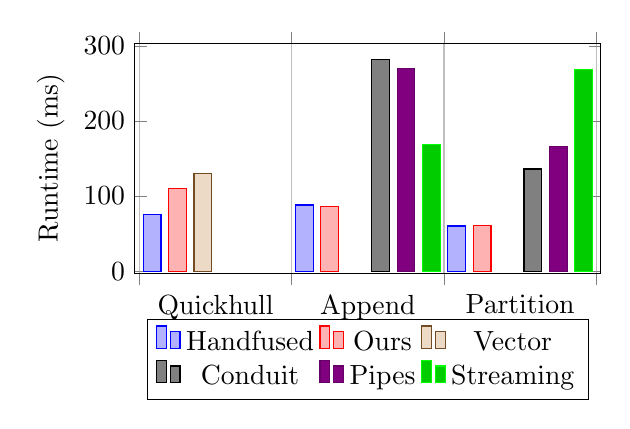
\begin{tikzpicture}
\begin{axis}[
  symbolic x coords={Quickhull, Append, Partition, end},
        ylabel=Runtime (ms),
  ymin=0, ymax=300,
        enlargelimits=0.01,
        ybar interval=0.7,
  width=7.5cm, height=4.5cm,
  legend style={at={(0.5,-0.2)},anchor=north, legend columns=3}
]
\addplot coordinates { (Quickhull, 75) (Append, 88) (Partition, 60) (end, 0) };
\addplot coordinates {(Quickhull, 110) (Append, 86) (Partition, 61) (end,0)};
\addplot coordinates { (Quickhull, 130) (Append, 0)  };
% \addplot coordinates { (Quickhull, 200) (Append, 0) };
\addplot coordinates {  (Append, 282) (Partition, 136) (end,0) };
\addplot coordinates {  (Append, 270) (Partition, 166) (end,0) };
\addplot coordinates {  (Append, 168) (Partition, 268) (end,0) };
\legend{Handfused, Ours, Vector, Conduit, Pipes, Streaming}
\end{axis}
\end{tikzpicture}
\caption{Runtime for benchmarks; lower is faster.}
\label{fig:bench:all}
\end{figure}

% Quickhull
% \addplot coordinates {(200,Store) (130,Recompute) (110,Ours) (75,Hand) (0,end) };
% Append
% \addplot coordinates {(282,Conduit) (270,Pipes) (168,Streaming) (86,Ours) (0,end) };
% Partition
% \addplot coordinates {(1200,Streaming) (764,Pipes) (658,Conduit hand) (288,Ours) (0,end) };


\input{section/05A-Benchmarks.tex}
%!TEX root = ../Main.tex

\section{Proofs}
\label{s:Proofs}

Our fusion system is formalised in Coq, where we have proved soundness of \ti{fusePair}: if the fused program evaluates to a particular output, then the two original programs also evaluate to that output.
It is interesting to note that the converse is not necessarily true: just because two programs can evaluate to a particular output does not mean the fused program will evaluate to that.
This is because, as explained in~\S\ref{s:EvaluationOrder}, evaluation of a process network is non-deterministic, and fusion commits to a particular evaluation order.

The system described here has some differences to our Coq formalisation.
First, the Coq formalisation has a separate @update@ instruction which modifies a variable in the local heap, rather than allowing heap updates in the output \Next~label of any instruction.
This causes the fusion definition to be slightly more complicated, as two output instructions must be emitted when performing a push or pull followed by an update.
This is a fairly minor difference, and we have made this change in the paper version for ease of exposition.
Ideally, a future version of the formalisation would include this change.
Secondly, our formalisation does not implement the concurrent evaluation semantics for processes, only sequential evaluation for a single process.
Instead we sequentially evaluate both processes separately with the same input values and outputs.

Despite these differences, we believe the Coq formalisation gives sufficient confidence in the correctness of the version presented here.


%!TEX root = ../Main.tex
\eject
\section{Related Work}
\label{s:Conclusion}

% This paper has introduced Icicle, a streaming query language. The streaming, single-pass nature of Icicle allows all queries over the same table to be fused into a single loop over the data.
% Icicle's modal type system allows incremental computation, ensuring that queries give the same value regardless of how the input is sliced up, and when the increments are performed.
% The modal types encode when computations are available, and disallows using the results of folds before they are finished.
% \ben{the above paragraph doesn't add any new information}.

In Icicle there is only one stream, sourced from the input table, which is implicit in the bodies of queries. This approach is intentionally simpler than existing synchronous data flow languages such as Lucy~\cite{mandel2010lucy}, as well as our prior work on flow fusion~\cite{lippmeier2013data}. Synchronous data flow languages implement Kahn networks~\cite{vrba2009kahn} that are restricted to use bounded buffering~\cite{johnston2004advances} by clock typing and causal analysis~\cite{stephens1997survey}. In such languages, stream combinators with multiple inputs, such as @zip@, are assigned types that require their stream arguments to have the same clock --- meaning that elements always arrive in lockstep and the combinators themselves do not need to perform their own buffering. In Icicle the fact that the input stream is implicit and distributed to all combinators means that we can forgo clock analysis. All queries in a program execute in lock-step on the same element at the same moment, which ensures that fusion is a simple matter of concatenating the components of the loop anatomy of each query.

Short-cut fusion techniques such as foldr/build~\cite{gill1993short} and stream fusion~\cite{coutts2007stream} rely on inlining to expose fusion opportunities. In Haskell compilers such as GHC, the decision of when to inline is made by internal compiler heuristics, which makes it difficult for the programmer to predict when fusion will occur. In this environment, array fusion is considered a ``bonus'' optimization rather than integral part of the compilation method. In contrast, for our feature generation application we really must ensure that multiple queries over the same table are fused, so we cannot rely on heuristics.

StreamIt~\cite{thies2002streamit} is an imperative streaming language which has been extended with dynamic scheduling~\cite{soule2013dynamic}. Dynamic scheduling handles data flow graphs where the transfer rate between different stream operators is not known at compile time. Dynamic scheduling is trade-off: it is required for stream operators such as grouping and filtering where the output data rate is not known statically, but using dynamic techniques for graphs with static transfer rates tends to have a performance cost. Icicle includes grouping and filtering operators where the output rates are statically unknown, however the associated language constructs require grouped and filtered data to be aggregated rather than passed as as the input to another stream operator. This allows Icicle to retain fully static scheduling, so the compiled queries consist of straight line code with no buffering.

Icicle is closely related to work in continuous and shared queries. A continuous query is one that processes input data which may have new records added or removed from it at any time. The result of the continuous query must be updated as soon as the input data changes. Shared queries are ones in which the same sub expressions occur in several individual queries over the same data, and we wish to share the results of these sub expressions among all individuals that use them. For example, in Munagala \emph{et al}~\cite{munagala2007optimization}, input records are filtered by a conjunction of predicates, and the predicates occur in multiple queries. Madden \emph{et al}~\cite{madden2002continuously} uses a predicate index to avoid recomputing them. Andrade \emph{et al} describes a compiler for queries over geospacial imagery~\cite{andrade2003efficient} that shares the results of several pre-defined aggregation functions between queries. Continuous Query Language (CQL)~\cite{arasu2002abstract,stream2003stream} again allows aggregates in its queries, but they must be builtin aggregate functions. Icicle addresses a computationally similar problem, except that our input data sets can only have new records added rather than deleted, which allows us to support general aggregations rather than just filter predicates. It is not obvious how arbitrary aggregate functions could be supported while also allowing deletion of records from the input data --- other than by recomputing the entire aggregation after each deletion.



% How to architect a query compiler~\cite{shaikhha2016architect}.
% Scheduling dynamic dataflow~\cite{buck1993scheduling}.
% Co-iterative characterization~\cite{caspi1998co}.

%!TEX root = ../Main.tex
\section{Extensions and future work}
\label{s:FutureWork}

We now discuss some of the shortcomings of the system, and extensions and future work to ameliorate this.

\subsection{Finite streams}
\label{s:Finite}

The processes we have seen so far deal with infinite streams, but in practice most streams are finite.
Certain combinators such as @fold@ and @append@ only make sense on finite streams, and others like @take@ produce inherently finite output.
We have focussed on the infinite stream version because it is somewhat simpler to explain and prove, but the extensions required to support finite streams do not require substantial conceptual changes.

We now describe the extensions required to support finite streams.
We add a new @closed@ constructor to the \InputState~ to encode the end of the stream.
Once an input stream is in the closed state, it can never change to another state: it remains closed thereafter.

We modify the @pull@ instruction so that it has two output labels (like @case@).
The first label, the read branch, is executed as before when the pull succeeds and a value is read from the stream.
The second label, the close branch, is executed when the stream is closed, and no more values will ever be available.
After a pull takes the close branch, any subsequent pulls from that stream will also take the close branch.

We add two new instructions for closing output streams and disconnecting from input streams.
Closing an output stream $(@close@~\Chan~\Goto)$ is similar to pushing an end-of-file marker to all readers.
As with @push@, the evaluation semantics of @close@ can only proceed if all readers are in a position to accept the end-of-file, but instead of setting the new \InputState~ to @pending@ with a value, the \InputState~ is set to @closed@.
After a stream has been closed, no further values can be pushed.

Disconnecting from input streams $(@disconnect@~\Chan~\Goto)$ signals that a process is no longer interested in the values of a stream.
This can be used when a process requires the first values of a stream, but does not require the whole stream.
If a process read the first values of a stream and then stopped pulling, its \InputState~ buffer would fill up and never be cleared, so no other process would be able to continue pulling from that stream.
Disconnecting the stream allows other processes to use the stream without the disconnected process getting in the way of computation.
The evaluation semantics for @disconnect@ remove the channel from the inputs of the process.
After removing the channel from the inputs, when a writing process tries to inject values, this process will just be ignored rather than inserting into the \InputState~ buffer and potentially causing writing to block.
After a process disconnects from an input channel, it can no longer pull from that channel.

We also add an instruction for terminating the process (@done@).
After all input streams have been read to completion or disconnected and output streams closed, the process may execute @done@ to signal that processing is complete.

The fusion definition must be extended to deal with these new instructions.
The static input state has a @closed@ constructor added and disconnection is encoded by removal from the input state, and the \ti{tryStep} changes more or less follow the evaluation changes.
Shared and connected pulls now deal with two more possibilities in the input state: the input may be closed in which case the close branch of the pull is taken; or the other process may have disconnected in which case the pull is executed as in the non-shared non-connected case.
Connected pushes must also deal with when the other process has disconnected in which case the push is executed as if it were non-connected.
For @in1@ and @out1@ channels, the new @close@ and @disconnect@ instructions are used as normal with no coordination required.
For connected @close@, as with @push@, the receiving process must have @none@ and the next step performs the @close@ and sets the input state to @closed@.
For shared @disconnect@, the @disconnect@ is only performed after both processes have disconnected; otherwise the entry is just removed from the input state.
For connected @disconnect@, the @disconnect@ is not performed and the entry is removed from the input state.

Finally, \ti{tryStepPair} is modified so that @done@ is performed when both machines are @done@.

These modifications allow our system to fuse finite streams as well as infinite.
We have implemented an initial prototype that supports finite streams, but future work is required to prove them correct.

\subsection{Fully abstract case interpretation}

This cannot be fused because it requires an unbounded buffer.
\begin{code}
zipltgts :: [a] -> [a*a]
zipltgts as =
  let as1 = filter (<0) as
      as2 = filter (>0) as
      aas = zip as1 as2
  in  aas
\end{code}

You might think the following can be fused.
It cannot because we treat @case@ conditions as fully abstract and make no attempt to filter out impossible combinations.
So while it cannot be true that the first filter reaches @>0 = true@ case and the second filter reaches @>0 = false@, we try both combinations and treat it as unfusable.
\begin{code}
zipgts :: [a] -> [a*a]
zipgts as =
  let as1 = filter (>0) as
      as2 = filter (>0) as
      aas = zip as1 as2
  in  aas
\end{code}


\bibliography{Main}

% %!TEX root = ../Main.tex
\appendix
\section{Combinators}
\label{s:Combinators}

Some simple combinator definitions.
Map 

\begin{code}
map f = stream_1_1 \is os.
  letrec
    p1   = pull is p2
    p2 i = push os (f i) p3
    p3   = drop is p1
  in p1
\end{code}

\begin{code}
filter f = stream_1_1 \is os.
  letrec
    p1   = pull is p2
    p2 i = case (f x) (p3 i) p4
    p3 i = push os i p4
    p4   = drop is p1
  in p1
\end{code}

\begin{code}
partition f = stream_1_2 \is ots ofs.
  letrec
    p1   = pull is p2
    p2 i = case (f x)
            (push ts i p3)
            (push fs i p3)
    p3   = drop is p1
  in p1
\end{code}

\begin{code}
zip = stream_2_1 \xs ys xys.
  letrec
    p1     = pull xs        p2
    p2 x   = pull ys        p3
    p3 x y = push xys (x,y) p4
    p4     = drop xs        p5
    p5     = drop ys        p1
  in p1
\end{code}


\begin{code}
merge = stream_2_1 \xs ys xys.
  letrec
    go x y = case (x < y)
             (pX x y)
             (pY x y)
    pX x y = push xys x
            (drop xs
            (pull xs (\x'. go x' y)))
    pY x y = push xys y
            (drop ys
            (pull ys (\y'. go x y')))
  in pull xs (\x. pull ys (\y. go x y))
\end{code}







\end{document}


